\documentclass{article}\usepackage[]{graphicx}\usepackage[]{color}
% maxwidth is the original width if it is less than linewidth
% otherwise use linewidth (to make sure the graphics do not exceed the margin)
\makeatletter
\def\maxwidth{ %
  \ifdim\Gin@nat@width>\linewidth
    \linewidth
  \else
    \Gin@nat@width
  \fi
}
\makeatother

\definecolor{fgcolor}{rgb}{0.345, 0.345, 0.345}
\newcommand{\hlnum}[1]{\textcolor[rgb]{0.686,0.059,0.569}{#1}}%
\newcommand{\hlstr}[1]{\textcolor[rgb]{0.192,0.494,0.8}{#1}}%
\newcommand{\hlcom}[1]{\textcolor[rgb]{0.678,0.584,0.686}{\textit{#1}}}%
\newcommand{\hlopt}[1]{\textcolor[rgb]{0,0,0}{#1}}%
\newcommand{\hlstd}[1]{\textcolor[rgb]{0.345,0.345,0.345}{#1}}%
\newcommand{\hlkwa}[1]{\textcolor[rgb]{0.161,0.373,0.58}{\textbf{#1}}}%
\newcommand{\hlkwb}[1]{\textcolor[rgb]{0.69,0.353,0.396}{#1}}%
\newcommand{\hlkwc}[1]{\textcolor[rgb]{0.333,0.667,0.333}{#1}}%
\newcommand{\hlkwd}[1]{\textcolor[rgb]{0.737,0.353,0.396}{\textbf{#1}}}%
\let\hlipl\hlkwb

\usepackage{framed}
\makeatletter
\newenvironment{kframe}{%
 \def\at@end@of@kframe{}%
 \ifinner\ifhmode%
  \def\at@end@of@kframe{\end{minipage}}%
  \begin{minipage}{\columnwidth}%
 \fi\fi%
 \def\FrameCommand##1{\hskip\@totalleftmargin \hskip-\fboxsep
 \colorbox{shadecolor}{##1}\hskip-\fboxsep
     % There is no \\@totalrightmargin, so:
     \hskip-\linewidth \hskip-\@totalleftmargin \hskip\columnwidth}%
 \MakeFramed {\advance\hsize-\width
   \@totalleftmargin\z@ \linewidth\hsize
   \@setminipage}}%
 {\par\unskip\endMakeFramed%
 \at@end@of@kframe}
\makeatother

\definecolor{shadecolor}{rgb}{.97, .97, .97}
\definecolor{messagecolor}{rgb}{0, 0, 0}
\definecolor{warningcolor}{rgb}{1, 0, 1}
\definecolor{errorcolor}{rgb}{1, 0, 0}
\newenvironment{knitrout}{}{} % an empty environment to be redefined in TeX

\usepackage{alltt}
\usepackage{Sweave}
\usepackage{float}
\usepackage{subcaption}
\usepackage{graphicx}
\usepackage{tabularx}
\usepackage{siunitx}
\usepackage{multirow}
\usepackage{amssymb} % for math symbols
\usepackage{amsmath} % for aligning equations
%\usepackage{hyperref}
\usepackage{textcomp}
\usepackage{mdframed}
\usepackage{longtable}
\usepackage{natbib}
\bibliographystyle{..//bib/styles/gcb}
%\usepackage[hyphens]{url}
\usepackage{caption}
\setlength{\captionmargin}{30pt}
\setlength{\abovecaptionskip}{0pt}
\setlength{\belowcaptionskip}{10pt}
\topmargin -1.5cm        
\oddsidemargin -0.04cm   
\evensidemargin -0.04cm
\textwidth 16.59cm
\textheight 21.94cm 
%\pagestyle{empty} %comment if want page numbers
\parskip 7.2pt
\renewcommand{\baselinestretch}{1}
\parindent 0pt
\usepackage{lineno}
\linenumbers

%cross referencing:
\usepackage{xr}
\externaldocument{regrisk}

\newmdenv[
  topline=true,
  bottomline=true,
  skipabove=\topsep,
  skipbelow=\topsep
]{siderules}

%% R Script


\IfFileExists{upquote.sty}{\usepackage{upquote}}{}
\begin{document}

\noindent \textbf{\Large{Supplemental materials: False spring damage on temperate tree seedlings is amplified with winter warming}}

\noindent Authors:\\
C. J. Chamberlain $^{1,2}$, K. Woodruff $^{1}$ \& E. M. Wolkovich $^{1,2,3}$
\vspace{2ex}\\
\emph{Author affiliations:}\\
$^{1}$Arnold Arboretum of Harvard University, 1300 Centre Street, Boston, Massachusetts, USA; \\
$^{2}$Organismic \& Evolutionary Biology, Harvard University, 26 Oxford Street, Cambridge, Massachusetts, USA; \\
$^{3}$Forest \& Conservation Sciences, Faculty of Forestry, University of British Columbia, 2424 Main Mall, Vancouver, BC V6T 1Z4\\
\vspace{2ex}
$^*$Corresponding author: 248.953.0189; cchamberlain@g.harvard.edu\\

\renewcommand{\thetable}{S\arabic{table}}
\renewcommand{\thefigure}{S\arabic{figure}}
\renewcommand{\labelitemi}{$-$}
\setkeys{Gin}{width=0.8\textwidth}

\section*{Supplemental Tables and Figures}




{\begin{figure} [H]
  -\begin{center}
  -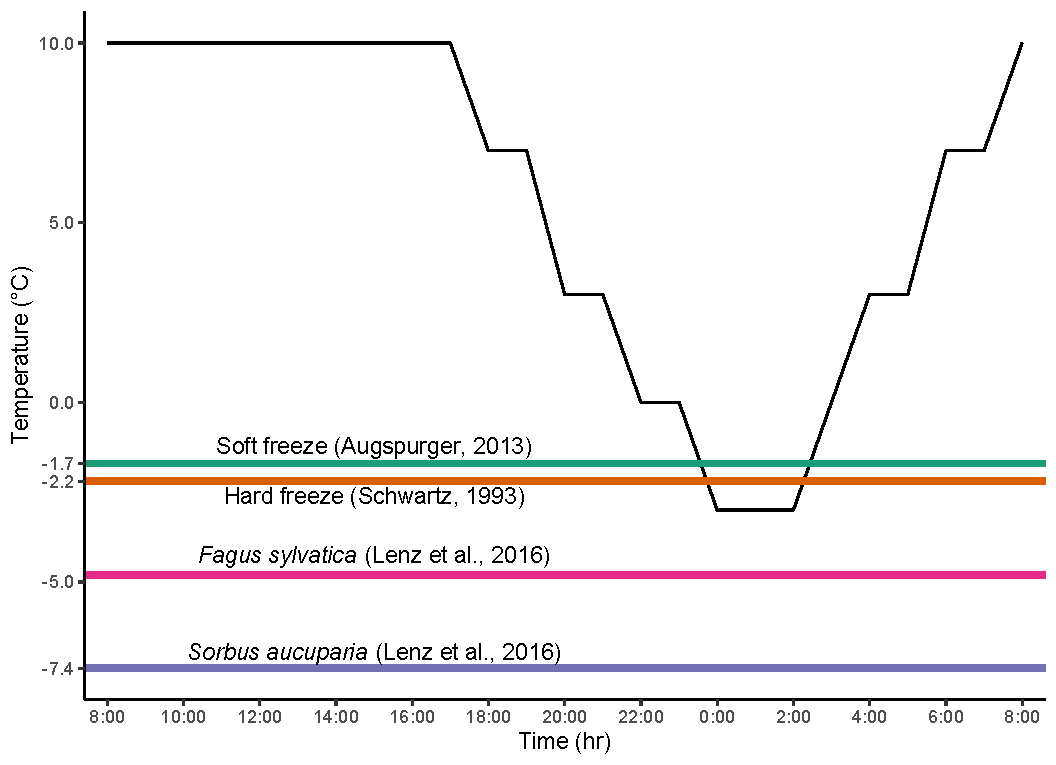
\includegraphics[width=12cm]{..//analyses/figures/growthchamber.pdf}%\label{fig:gccond}
  -\end{center}
  -\end{figure}}

\begin{kframe}


{\ttfamily\noindent\bfseries\color{errorcolor}{\#\# Error in gsub("{}r\_species["{}, "{}"{}, modoutput\$term): invalid regular expression 'r\_species[', reason 'Missing ']''}}\end{kframe}% latex table generated in R 3.6.0 by xtable 1.8-4 package
% Tue Mar 24 17:08:21 2020
\begin{longtable}{lrrrrrrr}
\caption{Summary of model with the effects of false spring treatment and chilling duration across species on duration of vegetative risk.} \\ 
  \hline
 & mean & 2\% & 10\% & 25\% & 75\% & 90\% & 98\% \\ 
  \hline \endhead  \hline
Intercept & 16.02 & 12.46 & 13.60 & 15.08 & 16.90 & 18.52 & 20.23 \\ 
  Tx & 2.97 & 1.13 & 1.68 & 2.45 & 3.49 & 4.26 & 4.87 \\ 
  Chill 6 Wks & -0.53 & -3.83 & -2.73 & -1.38 & 0.32 & 1.72 & 2.99 \\ 
  Chill 8 Wks & -2.67 & -5.54 & -4.56 & -3.35 & -1.94 & -0.85 & 0.03 \\ 
  Tx:Chill 6 Wks & -0.91 & -3.59 & -2.78 & -1.65 & -0.17 & 0.92 & 1.85 \\ 
  Tx:Chill 8 Wks & 0.62 & -1.97 & -1.14 & -0.08 & 1.34 & 2.38 & 3.25 \\ 
  r_species[\textit{Acer saccharinum},Intercept & -3.06 & -7.74 & -5.82 & -4.12 & -1.93 & -0.40 & 0.75 \\ 
  r_species[\textit{Alnus incana rugosa},Intercept & 4.39 & 0.17 & 1.66 & 3.33 & 5.44 & 7.19 & 8.51 \\ 
  r_species[\textit{Betula papyrifera},Intercept & 0.96 & -3.52 & -1.86 & -0.06 & 2.02 & 3.69 & 4.85 \\ 
  r_species[\textit{Betula populifolia},Intercept & 0.20 & -4.12 & -2.47 & -0.86 & 1.27 & 2.93 & 4.19 \\ 
  r_species[\textit{Cornus racemosa},Intercept & 0.48 & -3.87 & -2.35 & -0.54 & 1.57 & 3.10 & 4.26 \\ 
  r_species[\textit{Salix purpurea},Intercept & -5.49 & -10.38 & -8.46 & -6.57 & -4.33 & -2.69 & -1.40 \\ 
  r_species[\textit{Sorbus americana},Intercept & -1.14 & -5.56 & -3.88 & -2.20 & -0.07 & 1.60 & 2.79 \\ 
  r_species[\textit{Viburnum dendatum},Intercept & 3.57 & -0.78 & 0.80 & 2.51 & 4.67 & 6.29 & 7.69 \\ 
  r_species[\textit{Acer saccharinum},Tx & -0.36 & -2.80 & -1.82 & -0.72 & 0.05 & 0.63 & 1.27 \\ 
  r_species[\textit{Alnus incana rugosa},Tx & 0.37 & -1.36 & -0.73 & -0.06 & 0.76 & 1.91 & 2.86 \\ 
  r_species[\textit{Betula papyrifera},Tx & 0.45 & -1.17 & -0.54 & -0.03 & 0.84 & 2.03 & 3.08 \\ 
  r_species[\textit{Betula populifolia},Tx & -0.43 & -3.09 & -1.97 & -0.80 & 0.04 & 0.55 & 1.12 \\ 
  r_species[\textit{Cornus racemosa},Tx & 0.00 & -1.93 & -1.15 & -0.29 & 0.32 & 1.13 & 1.91 \\ 
  r_species[\textit{Salix purpurea},Tx & -0.14 & -2.48 & -1.59 & -0.55 & 0.25 & 1.21 & 2.14 \\ 
  r_species[\textit{Sorbus americana},Tx & -0.21 & -2.43 & -1.57 & -0.54 & 0.15 & 0.84 & 1.57 \\ 
  r_species[\textit{Viburnum dendatum},Tx & 0.35 & -1.38 & -0.75 & -0.10 & 0.74 & 1.93 & 2.86 \\ 
  r_species[\textit{Acer saccharinum},Chill 6 Wks & -0.13 & -4.23 & -2.82 & -1.21 & 0.92 & 2.61 & 4.04 \\ 
  r_species[\textit{Alnus incana rugosa},Chill 6 Wks & -0.66 & -4.71 & -3.50 & -1.71 & 0.41 & 2.10 & 3.53 \\ 
  r_species[\textit{Betula papyrifera},Chill 6 Wks & 1.50 & -2.35 & -1.14 & 0.40 & 2.54 & 4.30 & 5.65 \\ 
  r_species[\textit{Betula populifolia},Chill 6 Wks & -0.59 & -4.77 & -3.43 & -1.62 & 0.50 & 2.10 & 3.22 \\ 
  r_species[\textit{Cornus racemosa},Chill 6 Wks & 0.46 & -3.46 & -2.14 & -0.56 & 1.48 & 3.11 & 4.43 \\ 
  r_species[\textit{Salix purpurea},Chill 6 Wks & 4.60 & 0.55 & 1.62 & 3.26 & 5.84 & 7.88 & 9.27 \\ 
  r_species[\textit{Sorbus americana},Chill 6 Wks & -2.20 & -6.59 & -5.11 & -3.27 & -1.02 & 0.45 & 1.44 \\ 
  r_species[\textit{Viburnum dendatum},Chill 6 Wks & -3.19 & -7.67 & -6.24 & -4.28 & -2.01 & -0.48 & 0.62 \\ 
  r_species[\textit{Acer saccharinum},Chill 8 Wks & 0.94 & -2.40 & -1.30 & -0.02 & 1.85 & 3.42 & 4.57 \\ 
  r_species[\textit{Alnus incana rugosa},Chill 8 Wks & -1.32 & -5.07 & -3.77 & -2.23 & -0.38 & 1.04 & 2.09 \\ 
  r_species[\textit{Betula papyrifera},Chill 8 Wks & 0.21 & -3.49 & -2.22 & -0.68 & 1.12 & 2.52 & 3.77 \\ 
  r_species[\textit{Betula populifolia},Chill 8 Wks & -1.36 & -5.28 & -3.90 & -2.25 & -0.39 & 0.82 & 1.82 \\ 
  r_species[\textit{Cornus racemosa},Chill 8 Wks & 0.61 & -2.76 & -1.58 & -0.30 & 1.48 & 2.94 & 4.23 \\ 
  r_species[\textit{Salix purpurea},Chill 8 Wks & 3.91 & 0.30 & 1.23 & 2.72 & 5.00 & 6.79 & 8.30 \\ 
  r_species[\textit{Sorbus americana},Chill 8 Wks & -0.51 & -4.16 & -2.86 & -1.41 & 0.41 & 1.76 & 2.89 \\ 
  r_species[\textit{Viburnum dendatum},Chill 8 Wks & -2.54 & -6.43 & -5.09 & -3.50 & -1.50 & -0.18 & 0.69 \\ 
  r_species[\textit{Acer saccharinum},Tx:Chill 6 Wks & -0.46 & -4.34 & -2.80 & -0.98 & 0.16 & 1.15 & 2.08 \\ 
  r_species[\textit{Alnus incana rugosa},Tx:Chill 6 Wks & 0.35 & -2.54 & -1.42 & -0.27 & 0.89 & 2.66 & 4.38 \\ 
  r_species[\textit{Betula papyrifera},Tx:Chill 6 Wks & 0.33 & -2.71 & -1.36 & -0.22 & 0.85 & 2.44 & 3.77 \\ 
  r_species[\textit{Betula populifolia},Tx:Chill 6 Wks & -0.54 & -4.45 & -2.83 & -1.05 & 0.11 & 1.06 & 2.03 \\ 
  r_species[\textit{Cornus racemosa},Tx:Chill 6 Wks & 0.23 & -2.65 & -1.45 & -0.26 & 0.69 & 2.25 & 3.58 \\ 
  r_species[\textit{Salix purpurea},Tx:Chill 6 Wks & 1.07 & -1.87 & -0.80 & 0.02 & 1.84 & 4.03 & 5.96 \\ 
  r_species[\textit{Sorbus americana},Tx:Chill 6 Wks & -0.44 & -3.99 & -2.60 & -0.97 & 0.16 & 1.13 & 2.24 \\ 
  r_species[\textit{Viburnum dendatum},Tx:Chill 6 Wks & -0.58 & -4.61 & -2.97 & -1.16 & 0.10 & 1.07 & 2.17 \\ 
  r_species[\textit{Acer saccharinum},Tx:Chill 8 Wks & -0.05 & -2.85 & -1.67 & -0.45 & 0.33 & 1.47 & 2.79 \\ 
  r_species[\textit{Alnus incana rugosa},Tx:Chill 8 Wks & 0.12 & -2.75 & -1.46 & -0.30 & 0.54 & 1.87 & 3.40 \\ 
  r_species[\textit{Betula papyrifera},Tx:Chill 8 Wks & 0.31 & -1.95 & -1.01 & -0.16 & 0.72 & 2.14 & 3.56 \\ 
  r_species[\textit{Betula populifolia},Tx:Chill 8 Wks & -0.06 & -2.98 & -1.62 & -0.43 & 0.33 & 1.43 & 2.66 \\ 
  r_species[\textit{Cornus racemosa},Tx:Chill 8 Wks & 0.40 & -1.62 & -0.83 & -0.10 & 0.75 & 2.28 & 3.86 \\ 
  r_species[\textit{Salix purpurea},Tx:Chill 8 Wks & -0.09 & -3.49 & -2.09 & -0.58 & 0.43 & 1.75 & 2.95 \\ 
  r_species[\textit{Sorbus americana},Tx:Chill 8 Wks & -0.48 & -4.01 & -2.61 & -0.90 & 0.08 & 0.80 & 1.61 \\ 
  r_species[\textit{Viburnum dendatum},Tx:Chill 8 Wks & -0.25 & -3.57 & -2.24 & -0.67 & 0.26 & 1.25 & 2.36 \\ 
   \hline
\hline
\label{tab:suppmoddvr}
\end{longtable}


\newpage
\begin{kframe}


{\ttfamily\noindent\bfseries\color{errorcolor}{\#\# Error in file(file, "{}rt"{}): cannot open the connection}}

{\ttfamily\noindent\bfseries\color{errorcolor}{\#\# Error in `\$<-.data.frame`(`*tmp*`, term, value = character(0)): replacement has 0 rows, data has 54}}

{\ttfamily\noindent\bfseries\color{errorcolor}{\#\# Error in gsub("{}r\_species["{}, "{}"{}, modoutput\$term): invalid regular expression 'r\_species[', reason 'Missing ']''}}

{\ttfamily\noindent\bfseries\color{errorcolor}{\#\# Error in `\$<-.data.frame`(`*tmp*`, term, value = character(0)): replacement has 0 rows, data has 54}}

{\ttfamily\noindent\bfseries\color{errorcolor}{\#\# Error in `\$<-.data.frame`(`*tmp*`, term, value = character(0)): replacement has 0 rows, data has 54}}

{\ttfamily\noindent\bfseries\color{errorcolor}{\#\# Error in `\$<-.data.frame`(`*tmp*`, term, value = character(0)): replacement has 0 rows, data has 54}}

{\ttfamily\noindent\bfseries\color{errorcolor}{\#\# Error in `\$<-.data.frame`(`*tmp*`, term, value = character(0)): replacement has 0 rows, data has 54}}

{\ttfamily\noindent\bfseries\color{errorcolor}{\#\# Error in `\$<-.data.frame`(`*tmp*`, term, value = character(0)): replacement has 0 rows, data has 54}}

{\ttfamily\noindent\bfseries\color{errorcolor}{\#\# Error in `\$<-.data.frame`(`*tmp*`, term, value = character(0)): replacement has 0 rows, data has 54}}

{\ttfamily\noindent\bfseries\color{errorcolor}{\#\# Error in `\$<-.data.frame`(`*tmp*`, term, value = character(0)): replacement has 0 rows, data has 54}}

{\ttfamily\noindent\bfseries\color{errorcolor}{\#\# Error in `\$<-.data.frame`(`*tmp*`, term, value = character(0)): replacement has 0 rows, data has 54}}

{\ttfamily\noindent\bfseries\color{errorcolor}{\#\# Error in `\$<-.data.frame`(`*tmp*`, term, value = character(0)): replacement has 0 rows, data has 54}}

{\ttfamily\noindent\bfseries\color{errorcolor}{\#\# Error in `\$<-.data.frame`(`*tmp*`, term, value = character(0)): replacement has 0 rows, data has 54}}

{\ttfamily\noindent\bfseries\color{errorcolor}{\#\# Error in `\$<-.data.frame`(`*tmp*`, term, value = character(0)): replacement has 0 rows, data has 54}}

{\ttfamily\noindent\bfseries\color{errorcolor}{\#\# Error in `\$<-.data.frame`(`*tmp*`, term, value = character(0)): replacement has 0 rows, data has 54}}

{\ttfamily\noindent\bfseries\color{errorcolor}{\#\# Error in `\$<-.data.frame`(`*tmp*`, term, value = character(0)): replacement has 0 rows, data has 54}}

{\ttfamily\noindent\bfseries\color{errorcolor}{\#\# Error in `\$<-.data.frame`(`*tmp*`, term, value = character(0)): replacement has 0 rows, data has 54}}

{\ttfamily\noindent\bfseries\color{errorcolor}{\#\# Error in `\$<-.data.frame`(`*tmp*`, term, value = character(0)): replacement has 0 rows, data has 54}}\end{kframe}% latex table generated in R 3.6.0 by xtable 1.8-4 package
% Tue Mar 24 17:08:21 2020
\begin{longtable}{lrrrrrrr}
\caption{Summary of model with the effects of false spring treatment and chilling duration across species on growing season length.} \\ 
  \hline
 & mean & 2\% & 10\% & 25\% & 75\% & 90\% & 98\% \\ 
  \hline \endhead  \hline
Intercept & 16.02 & 12.46 & 13.60 & 15.08 & 16.90 & 18.52 & 20.23 \\ 
  Tx & 2.97 & 1.13 & 1.68 & 2.45 & 3.49 & 4.26 & 4.87 \\ 
  Chill 6 Wks & -0.53 & -3.83 & -2.73 & -1.38 & 0.32 & 1.72 & 2.99 \\ 
  Chill 8 Wks & -2.67 & -5.54 & -4.56 & -3.35 & -1.94 & -0.85 & 0.03 \\ 
  Tx:Chill 6 Wks & -0.91 & -3.59 & -2.78 & -1.65 & -0.17 & 0.92 & 1.85 \\ 
  Tx:Chill 8 Wks & 0.62 & -1.97 & -1.14 & -0.08 & 1.34 & 2.38 & 3.25 \\ 
  r_species[\textit{Sorbus americana},Chill 6 Wks & -2.20 & -6.59 & -5.11 & -3.27 & -1.02 & 0.45 & 1.44 \\ 
  r_species[\textit{Viburnum dendatum},Chill 6 Wks & -3.19 & -7.67 & -6.24 & -4.28 & -2.01 & -0.48 & 0.62 \\ 
  r_species[\textit{Acer saccharinum},Chill 8 Wks & 0.94 & -2.40 & -1.30 & -0.02 & 1.85 & 3.42 & 4.57 \\ 
  r_species[\textit{Alnus incana rugosa},Chill 8 Wks & -1.32 & -5.07 & -3.77 & -2.23 & -0.38 & 1.04 & 2.09 \\ 
  r_species[\textit{Betula papyrifera},Chill 8 Wks & 0.21 & -3.49 & -2.22 & -0.68 & 1.12 & 2.52 & 3.77 \\ 
  r_species[\textit{Betula populifolia},Chill 8 Wks & -1.36 & -5.28 & -3.90 & -2.25 & -0.39 & 0.82 & 1.82 \\ 
  r_species[\textit{Cornus racemosa},Chill 8 Wks & 0.61 & -2.76 & -1.58 & -0.30 & 1.48 & 2.94 & 4.23 \\ 
  r_species[\textit{Salix purpurea},Chill 8 Wks & 3.91 & 0.30 & 1.23 & 2.72 & 5.00 & 6.79 & 8.30 \\ 
  r_species[\textit{Sorbus americana},Chill 8 Wks & -0.51 & -4.16 & -2.86 & -1.41 & 0.41 & 1.76 & 2.89 \\ 
  r_species[\textit{Viburnum dendatum},Chill 8 Wks & -2.54 & -6.43 & -5.09 & -3.50 & -1.50 & -0.18 & 0.69 \\ 
  r_species[\textit{Acer saccharinum},Tx:Chill 6 Wks & -0.46 & -4.34 & -2.80 & -0.98 & 0.16 & 1.15 & 2.08 \\ 
  r_species[\textit{Alnus incana rugosa},Tx:Chill 6 Wks & 0.35 & -2.54 & -1.42 & -0.27 & 0.89 & 2.66 & 4.38 \\ 
  r_species[\textit{Betula papyrifera},Tx:Chill 6 Wks & 0.33 & -2.71 & -1.36 & -0.22 & 0.85 & 2.44 & 3.77 \\ 
  r_species[\textit{Betula populifolia},Tx:Chill 6 Wks & -0.54 & -4.45 & -2.83 & -1.05 & 0.11 & 1.06 & 2.03 \\ 
  r_species[\textit{Cornus racemosa},Tx:Chill 6 Wks & 0.23 & -2.65 & -1.45 & -0.26 & 0.69 & 2.25 & 3.58 \\ 
  r_species[\textit{Salix purpurea},Tx:Chill 6 Wks & 1.07 & -1.87 & -0.80 & 0.02 & 1.84 & 4.03 & 5.96 \\ 
  r_species[\textit{Sorbus americana},Tx:Chill 6 Wks & -0.44 & -3.99 & -2.60 & -0.97 & 0.16 & 1.13 & 2.24 \\ 
  r_species[\textit{Viburnum dendatum},Tx:Chill 6 Wks & -0.58 & -4.61 & -2.97 & -1.16 & 0.10 & 1.07 & 2.17 \\ 
  r_species[\textit{Acer saccharinum},Tx:Chill 8 Wks & -0.05 & -2.85 & -1.67 & -0.45 & 0.33 & 1.47 & 2.79 \\ 
  r_species[\textit{Alnus incana rugosa},Tx:Chill 8 Wks & 0.12 & -2.75 & -1.46 & -0.30 & 0.54 & 1.87 & 3.40 \\ 
  r_species[\textit{Betula papyrifera},Tx:Chill 8 Wks & 0.31 & -1.95 & -1.01 & -0.16 & 0.72 & 2.14 & 3.56 \\ 
  r_species[\textit{Betula populifolia},Tx:Chill 8 Wks & -0.06 & -2.98 & -1.62 & -0.43 & 0.33 & 1.43 & 2.66 \\ 
  r_species[\textit{Cornus racemosa},Tx:Chill 8 Wks & 0.40 & -1.62 & -0.83 & -0.10 & 0.75 & 2.28 & 3.86 \\ 
  r_species[\textit{Salix purpurea},Tx:Chill 8 Wks & -0.09 & -3.49 & -2.09 & -0.58 & 0.43 & 1.75 & 2.95 \\ 
  r_species[\textit{Sorbus americana},Tx:Chill 8 Wks & -0.48 & -4.01 & -2.61 & -0.90 & 0.08 & 0.80 & 1.61 \\ 
  r_species[\textit{Viburnum dendatum},Tx:Chill 8 Wks & -0.25 & -3.57 & -2.24 & -0.67 & 0.26 & 1.25 & 2.36 \\ 
   &  &  &  &  &  &  &  \\ 
   &  &  &  &  &  &  &  \\ 
   &  &  &  &  &  &  &  \\ 
   &  &  &  &  &  &  &  \\ 
   &  &  &  &  &  &  &  \\ 
   &  &  &  &  &  &  &  \\ 
   &  &  &  &  &  &  &  \\ 
   &  &  &  &  &  &  &  \\ 
   &  &  &  &  &  &  &  \\ 
   &  &  &  &  &  &  &  \\ 
   &  &  &  &  &  &  &  \\ 
   &  &  &  &  &  &  &  \\ 
   &  &  &  &  &  &  &  \\ 
   &  &  &  &  &  &  &  \\ 
   &  &  &  &  &  &  &  \\ 
   &  &  &  &  &  &  &  \\ 
   &  &  &  &  &  &  &  \\ 
   &  &  &  &  &  &  &  \\ 
   &  &  &  &  &  &  &  \\ 
   &  &  &  &  &  &  &  \\ 
   &  &  &  &  &  &  &  \\ 
   &  &  &  &  &  &  &  \\ 
   \hline
\hline
\label{tab:suppmodgs}
\end{longtable}



\newpage
\begin{kframe}


{\ttfamily\noindent\bfseries\color{errorcolor}{\#\# Error in file(file, "{}rt"{}): cannot open the connection}}

{\ttfamily\noindent\bfseries\color{errorcolor}{\#\# Error in `\$<-.data.frame`(`*tmp*`, term, value = character(0)): replacement has 0 rows, data has 54}}

{\ttfamily\noindent\bfseries\color{errorcolor}{\#\# Error in gsub("{}r\_species["{}, "{}"{}, modoutput\$term): invalid regular expression 'r\_species[', reason 'Missing ']''}}

{\ttfamily\noindent\bfseries\color{errorcolor}{\#\# Error in `\$<-.data.frame`(`*tmp*`, term, value = character(0)): replacement has 0 rows, data has 54}}

{\ttfamily\noindent\bfseries\color{errorcolor}{\#\# Error in `\$<-.data.frame`(`*tmp*`, term, value = character(0)): replacement has 0 rows, data has 54}}

{\ttfamily\noindent\bfseries\color{errorcolor}{\#\# Error in `\$<-.data.frame`(`*tmp*`, term, value = character(0)): replacement has 0 rows, data has 54}}

{\ttfamily\noindent\bfseries\color{errorcolor}{\#\# Error in `\$<-.data.frame`(`*tmp*`, term, value = character(0)): replacement has 0 rows, data has 54}}

{\ttfamily\noindent\bfseries\color{errorcolor}{\#\# Error in `\$<-.data.frame`(`*tmp*`, term, value = character(0)): replacement has 0 rows, data has 54}}

{\ttfamily\noindent\bfseries\color{errorcolor}{\#\# Error in `\$<-.data.frame`(`*tmp*`, term, value = character(0)): replacement has 0 rows, data has 54}}

{\ttfamily\noindent\bfseries\color{errorcolor}{\#\# Error in `\$<-.data.frame`(`*tmp*`, term, value = character(0)): replacement has 0 rows, data has 54}}

{\ttfamily\noindent\bfseries\color{errorcolor}{\#\# Error in `\$<-.data.frame`(`*tmp*`, term, value = character(0)): replacement has 0 rows, data has 54}}

{\ttfamily\noindent\bfseries\color{errorcolor}{\#\# Error in `\$<-.data.frame`(`*tmp*`, term, value = character(0)): replacement has 0 rows, data has 54}}

{\ttfamily\noindent\bfseries\color{errorcolor}{\#\# Error in `\$<-.data.frame`(`*tmp*`, term, value = character(0)): replacement has 0 rows, data has 54}}

{\ttfamily\noindent\bfseries\color{errorcolor}{\#\# Error in `\$<-.data.frame`(`*tmp*`, term, value = character(0)): replacement has 0 rows, data has 54}}

{\ttfamily\noindent\bfseries\color{errorcolor}{\#\# Error in `\$<-.data.frame`(`*tmp*`, term, value = character(0)): replacement has 0 rows, data has 54}}

{\ttfamily\noindent\bfseries\color{errorcolor}{\#\# Error in `\$<-.data.frame`(`*tmp*`, term, value = character(0)): replacement has 0 rows, data has 54}}

{\ttfamily\noindent\bfseries\color{errorcolor}{\#\# Error in `\$<-.data.frame`(`*tmp*`, term, value = character(0)): replacement has 0 rows, data has 54}}

{\ttfamily\noindent\bfseries\color{errorcolor}{\#\# Error in `\$<-.data.frame`(`*tmp*`, term, value = character(0)): replacement has 0 rows, data has 54}}\end{kframe}% latex table generated in R 3.6.0 by xtable 1.8-4 package
% Tue Mar 24 17:08:21 2020
\begin{longtable}{lrrrrrrr}
\caption{Summary of model with the effects of false spring treatment and chilling duration across species on shoot apical meristem growth.} \\ 
  \hline
 & mean & 2\% & 10\% & 25\% & 75\% & 90\% & 98\% \\ 
  \hline \endhead  \hline
Intercept & 16.02 & 12.46 & 13.60 & 15.08 & 16.90 & 18.52 & 20.23 \\ 
  Tx & 2.97 & 1.13 & 1.68 & 2.45 & 3.49 & 4.26 & 4.87 \\ 
  Chill 6 Wks & -0.53 & -3.83 & -2.73 & -1.38 & 0.32 & 1.72 & 2.99 \\ 
  Chill 8 Wks & -2.67 & -5.54 & -4.56 & -3.35 & -1.94 & -0.85 & 0.03 \\ 
  Tx:Chill 6 Wks & -0.91 & -3.59 & -2.78 & -1.65 & -0.17 & 0.92 & 1.85 \\ 
  Tx:Chill 8 Wks & 0.62 & -1.97 & -1.14 & -0.08 & 1.34 & 2.38 & 3.25 \\ 
  r_species[\textit{Cornus racemosa},Tx:Chill 8 Wks & 0.40 & -1.62 & -0.83 & -0.10 & 0.75 & 2.28 & 3.86 \\ 
  r_species[\textit{Salix purpurea},Tx:Chill 8 Wks & -0.09 & -3.49 & -2.09 & -0.58 & 0.43 & 1.75 & 2.95 \\ 
  r_species[\textit{Sorbus americana},Tx:Chill 8 Wks & -0.48 & -4.01 & -2.61 & -0.90 & 0.08 & 0.80 & 1.61 \\ 
  r_species[\textit{Viburnum dendatum},Tx:Chill 8 Wks & -0.25 & -3.57 & -2.24 & -0.67 & 0.26 & 1.25 & 2.36 \\ 
   &  &  &  &  &  &  &  \\ 
   &  &  &  &  &  &  &  \\ 
   &  &  &  &  &  &  &  \\ 
   &  &  &  &  &  &  &  \\ 
   &  &  &  &  &  &  &  \\ 
   &  &  &  &  &  &  &  \\ 
   &  &  &  &  &  &  &  \\ 
   &  &  &  &  &  &  &  \\ 
   &  &  &  &  &  &  &  \\ 
   &  &  &  &  &  &  &  \\ 
   &  &  &  &  &  &  &  \\ 
   &  &  &  &  &  &  &  \\ 
   &  &  &  &  &  &  &  \\ 
   &  &  &  &  &  &  &  \\ 
   &  &  &  &  &  &  &  \\ 
   &  &  &  &  &  &  &  \\ 
   &  &  &  &  &  &  &  \\ 
   &  &  &  &  &  &  &  \\ 
   &  &  &  &  &  &  &  \\ 
   &  &  &  &  &  &  &  \\ 
   &  &  &  &  &  &  &  \\ 
   &  &  &  &  &  &  &  \\ 
   &  &  &  &  &  &  &  \\ 
   &  &  &  &  &  &  &  \\ 
   &  &  &  &  &  &  &  \\ 
   &  &  &  &  &  &  &  \\ 
   &  &  &  &  &  &  &  \\ 
   &  &  &  &  &  &  &  \\ 
   &  &  &  &  &  &  &  \\ 
   &  &  &  &  &  &  &  \\ 
   &  &  &  &  &  &  &  \\ 
   &  &  &  &  &  &  &  \\ 
   &  &  &  &  &  &  &  \\ 
   &  &  &  &  &  &  &  \\ 
   &  &  &  &  &  &  &  \\ 
   &  &  &  &  &  &  &  \\ 
   &  &  &  &  &  &  &  \\ 
   &  &  &  &  &  &  &  \\ 
   &  &  &  &  &  &  &  \\ 
   &  &  &  &  &  &  &  \\ 
   &  &  &  &  &  &  &  \\ 
   &  &  &  &  &  &  &  \\ 
   &  &  &  &  &  &  &  \\ 
   &  &  &  &  &  &  &  \\ 
   \hline
\hline
\label{tab:suppmodmeri}
\end{longtable}



\newpage
\begin{kframe}


{\ttfamily\noindent\bfseries\color{errorcolor}{\#\# Error in gsub("{}r\_species["{}, "{}"{}, modoutput\$term): invalid regular expression 'r\_species[', reason 'Missing ']''}}\end{kframe}% latex table generated in R 3.6.0 by xtable 1.8-4 package
% Tue Mar 24 17:08:21 2020
\begin{longtable}{lrrrrrrr}
\caption{Summary of model with the effects of false spring treatment and chilling duration across species on leaf chlorophyll content.} \\ 
  \hline
 & mean & 2\% & 10\% & 25\% & 75\% & 90\% & 98\% \\ 
  \hline \endhead  \hline
Intercept & 30.16 & 23.88 & 26.03 & 28.65 & 31.70 & 34.08 & 36.04 \\ 
  Tx & -0.32 & -2.16 & -1.59 & -0.84 & 0.18 & 0.94 & 1.53 \\ 
  Chill 6 Wks & 0.11 & -1.86 & -1.20 & -0.45 & 0.66 & 1.49 & 2.22 \\ 
  Chill 8 Wks & 0.61 & -1.49 & -0.81 & 0.03 & 1.15 & 2.12 & 3.00 \\ 
  Tx:Chill 6 Wks & -0.82 & -3.42 & -2.69 & -1.61 & -0.07 & 1.14 & 2.12 \\ 
  Tx:Chill 8 Wks & -1.97 & -4.48 & -3.67 & -2.66 & -1.27 & -0.26 & 0.52 \\ 
  Intercept & 29.77 & 23.73 & 25.79 & 28.36 & 31.27 & 33.56 & 35.47 \\ 
  r_species[\textit{Acer saccharinum},Intercept & -5.14 & -11.39 & -9.18 & -6.71 & -3.62 & -0.95 & 1.16 \\ 
  r_species[\textit{Alnus incana rugosa},Intercept & 6.38 & 0.27 & 2.31 & 4.74 & 7.95 & 10.74 & 12.82 \\ 
  r_species[\textit{Betula papyrifera},Intercept & -1.61 & -7.66 & -5.57 & -3.24 & -0.08 & 2.62 & 4.70 \\ 
  r_species[\textit{Betula populifolia},Intercept & 1.40 & -4.47 & -2.63 & -0.23 & 2.88 & 5.66 & 7.77 \\ 
  r_species[\textit{Cornus racemosa},Intercept & 1.69 & -4.55 & -2.33 & 0.09 & 3.28 & 5.88 & 8.11 \\ 
  r_species[NYSSYL,Intercept & -2.28 & -11.59 & -8.71 & -4.83 & 0.34 & 3.97 & 6.94 \\ 
  r_species[\textit{Salix purpurea},Intercept & 12.96 & 6.80 & 8.90 & 11.28 & 14.54 & 17.38 & 19.44 \\ 
  r_species[\textit{Sorbus americana},Intercept & -6.48 & -12.54 & -10.51 & -8.10 & -4.90 & -2.28 & -0.09 \\ 
  r_species[\textit{Viburnum dendatum},Intercept & -4.13 & -10.23 & -8.19 & -5.71 & -2.58 & 0.12 & 2.31 \\ 
  r_species[\textit{Acer saccharinum},Tx & 0.02 & -1.90 & -1.00 & -0.24 & 0.30 & 1.03 & 1.74 \\ 
  r_species[\textit{Alnus incana rugosa},Tx & -0.06 & -1.95 & -1.21 & -0.34 & 0.22 & 0.99 & 1.83 \\ 
  r_species[\textit{Betula papyrifera},Tx & -0.23 & -2.52 & -1.50 & -0.48 & 0.09 & 0.64 & 1.23 \\ 
  r_species[\textit{Betula populifolia},Tx & -0.15 & -2.26 & -1.30 & -0.41 & 0.14 & 0.76 & 1.34 \\ 
  r_species[\textit{Cornus racemosa},Tx & 0.03 & -1.76 & -1.00 & -0.24 & 0.30 & 1.11 & 1.96 \\ 
  r_species[NYSSYL,Tx & 0.04 & -2.58 & -1.31 & -0.26 & 0.36 & 1.38 & 2.56 \\ 
  r_species[\textit{Salix purpurea},Tx & -0.47 & -3.24 & -2.13 & -0.88 & 0.04 & 0.61 & 1.26 \\ 
  r_species[\textit{Sorbus americana},Tx & 0.29 & -1.29 & -0.65 & -0.08 & 0.60 & 1.61 & 2.54 \\ 
  r_species[\textit{Viburnum dendatum},Tx & 0.28 & -1.16 & -0.59 & -0.06 & 0.58 & 1.56 & 2.37 \\ 
  r_species[\textit{Acer saccharinum},Chill 6 Wks & 0.29 & -1.96 & -1.05 & -0.16 & 0.74 & 1.85 & 2.94 \\ 
  r_species[\textit{Alnus incana rugosa},Chill 6 Wks & -0.70 & -4.26 & -2.80 & -1.23 & -0.00 & 0.62 & 1.35 \\ 
  r_species[\textit{Betula papyrifera},Chill 6 Wks & 0.56 & -1.37 & -0.62 & -0.03 & 1.02 & 2.45 & 3.73 \\ 
  r_species[\textit{Betula populifolia},Chill 6 Wks & 0.23 & -1.99 & -1.14 & -0.24 & 0.63 & 1.97 & 3.16 \\ 
  r_species[\textit{Cornus racemosa},Chill 6 Wks & -0.48 & -3.51 & -2.30 & -0.93 & 0.08 & 0.78 & 1.59 \\ 
  r_species[NYSSYL,Chill 6 Wks & 0.09 & -3.70 & -1.86 & -0.40 & 0.58 & 2.20 & 3.95 \\ 
  r_species[\textit{Salix purpurea},Chill 6 Wks & -0.85 & -4.26 & -3.04 & -1.46 & -0.03 & 0.56 & 1.36 \\ 
  r_species[\textit{Sorbus americana},Chill 6 Wks & 0.02 & -2.97 & -1.64 & -0.39 & 0.49 & 1.54 & 2.45 \\ 
  r_species[\textit{Viburnum dendatum},Chill 6 Wks & 0.26 & -2.02 & -1.09 & -0.18 & 0.71 & 1.83 & 2.87 \\ 
  r_species[\textit{Acer saccharinum},Chill 8 Wks & -0.05 & -2.81 & -1.71 & -0.50 & 0.42 & 1.54 & 2.39 \\ 
  r_species[\textit{Alnus incana rugosa},Chill 8 Wks & 0.25 & -2.45 & -1.31 & -0.26 & 0.77 & 2.01 & 3.18 \\ 
  r_species[\textit{Betula papyrifera},Chill 8 Wks & 0.10 & -2.66 & -1.47 & -0.36 & 0.56 & 1.76 & 2.77 \\ 
  r_species[\textit{Betula populifolia},Chill 8 Wks & -0.01 & -2.78 & -1.64 & -0.46 & 0.49 & 1.58 & 2.50 \\ 
  r_species[\textit{Cornus racemosa},Chill 8 Wks & 1.03 & -0.94 & -0.31 & 0.11 & 1.71 & 3.26 & 4.41 \\ 
  r_species[NYSSYL,Chill 8 Wks & -0.04 & -4.58 & -2.54 & -0.63 & 0.58 & 2.39 & 4.46 \\ 
  r_species[\textit{Salix purpurea},Chill 8 Wks & -0.43 & -3.85 & -2.59 & -1.00 & 0.25 & 1.22 & 2.06 \\ 
  r_species[\textit{Sorbus americana},Chill 8 Wks & -0.80 & -4.37 & -3.01 & -1.40 & -0.01 & 0.64 & 1.32 \\ 
  r_species[\textit{Viburnum dendatum},Chill 8 Wks & -0.80 & -4.46 & -2.97 & -1.36 & -0.02 & 0.56 & 1.24 \\ 
  r_species[\textit{Acer saccharinum},Tx:Chill 6 Wks & 0.03 & -3.29 & -1.89 & -0.48 & 0.59 & 1.84 & 2.91 \\ 
  r_species[\textit{Alnus incana rugosa},Tx:Chill 6 Wks & 0.07 & -3.15 & -1.94 & -0.54 & 0.59 & 2.27 & 3.94 \\ 
  r_species[\textit{Betula papyrifera},Tx:Chill 6 Wks & -0.09 & -3.57 & -2.04 & -0.57 & 0.48 & 1.63 & 2.82 \\ 
  r_species[\textit{Betula populifolia},Tx:Chill 6 Wks & -0.95 & -5.67 & -3.62 & -1.58 & -0.02 & 0.62 & 1.42 \\ 
  r_species[\textit{Cornus racemosa},Tx:Chill 6 Wks & 0.14 & -2.87 & -1.64 & -0.43 & 0.69 & 2.14 & 3.42 \\ 
  r_species[NYSSYL,Tx:Chill 6 Wks & 0.10 & -4.63 & -2.38 & -0.55 & 0.74 & 2.73 & 5.13 \\ 
  r_species[\textit{Salix purpurea},Tx:Chill 6 Wks & -1.34 & -6.10 & -4.38 & -2.27 & -0.12 & 0.61 & 1.50 \\ 
  r_species[\textit{Sorbus americana},Tx:Chill 6 Wks & 0.85 & -1.78 & -0.84 & 0.00 & 1.50 & 3.37 & 4.90 \\ 
  r_species[\textit{Viburnum dendatum},Tx:Chill 6 Wks & 0.20 & -3.03 & -1.62 & -0.35 & 0.75 & 2.15 & 3.38 \\ 
  r_species[\textit{Acer saccharinum},Tx:Chill 8 Wks & 0.01 & -2.43 & -1.28 & -0.29 & 0.32 & 1.26 & 2.33 \\ 
  r_species[\textit{Alnus incana rugosa},Tx:Chill 8 Wks & 0.03 & -2.19 & -1.30 & -0.28 & 0.36 & 1.30 & 2.38 \\ 
   \hline
\hline
\label{tab:suppmodchl}
\end{longtable}



\newpage
\begin{kframe}


{\ttfamily\noindent\bfseries\color{errorcolor}{\#\# Error in file(file, "{}rt"{}): cannot open the connection}}

{\ttfamily\noindent\bfseries\color{errorcolor}{\#\# Error in `\$<-.data.frame`(`*tmp*`, term, value = character(0)): replacement has 0 rows, data has 54}}

{\ttfamily\noindent\bfseries\color{errorcolor}{\#\# Error in gsub("{}r\_species["{}, "{}"{}, modoutput\$term): invalid regular expression 'r\_species[', reason 'Missing ']''}}

{\ttfamily\noindent\bfseries\color{errorcolor}{\#\# Error in `\$<-.data.frame`(`*tmp*`, term, value = character(0)): replacement has 0 rows, data has 54}}

{\ttfamily\noindent\bfseries\color{errorcolor}{\#\# Error in `\$<-.data.frame`(`*tmp*`, term, value = character(0)): replacement has 0 rows, data has 54}}

{\ttfamily\noindent\bfseries\color{errorcolor}{\#\# Error in `\$<-.data.frame`(`*tmp*`, term, value = character(0)): replacement has 0 rows, data has 54}}

{\ttfamily\noindent\bfseries\color{errorcolor}{\#\# Error in `\$<-.data.frame`(`*tmp*`, term, value = character(0)): replacement has 0 rows, data has 54}}

{\ttfamily\noindent\bfseries\color{errorcolor}{\#\# Error in `\$<-.data.frame`(`*tmp*`, term, value = character(0)): replacement has 0 rows, data has 54}}

{\ttfamily\noindent\bfseries\color{errorcolor}{\#\# Error in `\$<-.data.frame`(`*tmp*`, term, value = character(0)): replacement has 0 rows, data has 54}}

{\ttfamily\noindent\bfseries\color{errorcolor}{\#\# Error in `\$<-.data.frame`(`*tmp*`, term, value = character(0)): replacement has 0 rows, data has 54}}

{\ttfamily\noindent\bfseries\color{errorcolor}{\#\# Error in `\$<-.data.frame`(`*tmp*`, term, value = character(0)): replacement has 0 rows, data has 54}}

{\ttfamily\noindent\bfseries\color{errorcolor}{\#\# Error in `\$<-.data.frame`(`*tmp*`, term, value = character(0)): replacement has 0 rows, data has 54}}

{\ttfamily\noindent\bfseries\color{errorcolor}{\#\# Error in `\$<-.data.frame`(`*tmp*`, term, value = character(0)): replacement has 0 rows, data has 54}}

{\ttfamily\noindent\bfseries\color{errorcolor}{\#\# Error in `\$<-.data.frame`(`*tmp*`, term, value = character(0)): replacement has 0 rows, data has 54}}

{\ttfamily\noindent\bfseries\color{errorcolor}{\#\# Error in `\$<-.data.frame`(`*tmp*`, term, value = character(0)): replacement has 0 rows, data has 54}}

{\ttfamily\noindent\bfseries\color{errorcolor}{\#\# Error in `\$<-.data.frame`(`*tmp*`, term, value = character(0)): replacement has 0 rows, data has 54}}

{\ttfamily\noindent\bfseries\color{errorcolor}{\#\# Error in `\$<-.data.frame`(`*tmp*`, term, value = character(0)): replacement has 0 rows, data has 54}}

{\ttfamily\noindent\bfseries\color{errorcolor}{\#\# Error in `\$<-.data.frame`(`*tmp*`, term, value = character(0)): replacement has 0 rows, data has 54}}\end{kframe}% latex table generated in R 3.6.0 by xtable 1.8-4 package
% Tue Mar 24 17:08:21 2020
\begin{longtable}{lrrrrrrr}
\caption{Summary of model with the effects of false spring treatment and chilling duration across species on leaf toughness.} \\ 
  \hline
 & mean & 2\% & 10\% & 25\% & 75\% & 90\% & 98\% \\ 
  \hline \endhead  \hline
Intercept & 30.16 & 23.88 & 26.03 & 28.65 & 31.70 & 34.08 & 36.04 \\ 
  Tx & -0.32 & -2.16 & -1.59 & -0.84 & 0.18 & 0.94 & 1.53 \\ 
  Chill 6 Wks & 0.11 & -1.86 & -1.20 & -0.45 & 0.66 & 1.49 & 2.22 \\ 
  Chill 8 Wks & 0.61 & -1.49 & -0.81 & 0.03 & 1.15 & 2.12 & 3.00 \\ 
  Tx:Chill 6 Wks & -0.82 & -3.42 & -2.69 & -1.61 & -0.07 & 1.14 & 2.12 \\ 
  Tx:Chill 8 Wks & -1.97 & -4.48 & -3.67 & -2.66 & -1.27 & -0.26 & 0.52 \\ 
  r_species[\textit{Betula populifolia},Chill 6 Wks & 0.23 & -1.99 & -1.14 & -0.24 & 0.63 & 1.97 & 3.16 \\ 
  r_species[\textit{Cornus racemosa},Chill 6 Wks & -0.48 & -3.51 & -2.30 & -0.93 & 0.08 & 0.78 & 1.59 \\ 
  r_species[NYSSYL,Chill 6 Wks & 0.09 & -3.70 & -1.86 & -0.40 & 0.58 & 2.20 & 3.95 \\ 
  r_species[\textit{Salix purpurea},Chill 6 Wks & -0.85 & -4.26 & -3.04 & -1.46 & -0.03 & 0.56 & 1.36 \\ 
  r_species[\textit{Sorbus americana},Chill 6 Wks & 0.02 & -2.97 & -1.64 & -0.39 & 0.49 & 1.54 & 2.45 \\ 
  r_species[\textit{Viburnum dendatum},Chill 6 Wks & 0.26 & -2.02 & -1.09 & -0.18 & 0.71 & 1.83 & 2.87 \\ 
  r_species[\textit{Acer saccharinum},Chill 8 Wks & -0.05 & -2.81 & -1.71 & -0.50 & 0.42 & 1.54 & 2.39 \\ 
  r_species[\textit{Alnus incana rugosa},Chill 8 Wks & 0.25 & -2.45 & -1.31 & -0.26 & 0.77 & 2.01 & 3.18 \\ 
  r_species[\textit{Betula papyrifera},Chill 8 Wks & 0.10 & -2.66 & -1.47 & -0.36 & 0.56 & 1.76 & 2.77 \\ 
  r_species[\textit{Betula populifolia},Chill 8 Wks & -0.01 & -2.78 & -1.64 & -0.46 & 0.49 & 1.58 & 2.50 \\ 
  r_species[\textit{Cornus racemosa},Chill 8 Wks & 1.03 & -0.94 & -0.31 & 0.11 & 1.71 & 3.26 & 4.41 \\ 
  r_species[NYSSYL,Chill 8 Wks & -0.04 & -4.58 & -2.54 & -0.63 & 0.58 & 2.39 & 4.46 \\ 
  r_species[\textit{Salix purpurea},Chill 8 Wks & -0.43 & -3.85 & -2.59 & -1.00 & 0.25 & 1.22 & 2.06 \\ 
  r_species[\textit{Sorbus americana},Chill 8 Wks & -0.80 & -4.37 & -3.01 & -1.40 & -0.01 & 0.64 & 1.32 \\ 
  r_species[\textit{Viburnum dendatum},Chill 8 Wks & -0.80 & -4.46 & -2.97 & -1.36 & -0.02 & 0.56 & 1.24 \\ 
  r_species[\textit{Acer saccharinum},Tx:Chill 6 Wks & 0.03 & -3.29 & -1.89 & -0.48 & 0.59 & 1.84 & 2.91 \\ 
  r_species[\textit{Alnus incana rugosa},Tx:Chill 6 Wks & 0.07 & -3.15 & -1.94 & -0.54 & 0.59 & 2.27 & 3.94 \\ 
  r_species[\textit{Betula papyrifera},Tx:Chill 6 Wks & -0.09 & -3.57 & -2.04 & -0.57 & 0.48 & 1.63 & 2.82 \\ 
  r_species[\textit{Betula populifolia},Tx:Chill 6 Wks & -0.95 & -5.67 & -3.62 & -1.58 & -0.02 & 0.62 & 1.42 \\ 
  r_species[\textit{Cornus racemosa},Tx:Chill 6 Wks & 0.14 & -2.87 & -1.64 & -0.43 & 0.69 & 2.14 & 3.42 \\ 
  r_species[NYSSYL,Tx:Chill 6 Wks & 0.10 & -4.63 & -2.38 & -0.55 & 0.74 & 2.73 & 5.13 \\ 
  r_species[\textit{Salix purpurea},Tx:Chill 6 Wks & -1.34 & -6.10 & -4.38 & -2.27 & -0.12 & 0.61 & 1.50 \\ 
  r_species[\textit{Sorbus americana},Tx:Chill 6 Wks & 0.85 & -1.78 & -0.84 & 0.00 & 1.50 & 3.37 & 4.90 \\ 
  r_species[\textit{Viburnum dendatum},Tx:Chill 6 Wks & 0.20 & -3.03 & -1.62 & -0.35 & 0.75 & 2.15 & 3.38 \\ 
  r_species[\textit{Acer saccharinum},Tx:Chill 8 Wks & 0.01 & -2.43 & -1.28 & -0.29 & 0.32 & 1.26 & 2.33 \\ 
  r_species[\textit{Alnus incana rugosa},Tx:Chill 8 Wks & 0.03 & -2.19 & -1.30 & -0.28 & 0.36 & 1.30 & 2.38 \\ 
   &  &  &  &  &  &  &  \\ 
   &  &  &  &  &  &  &  \\ 
   &  &  &  &  &  &  &  \\ 
   &  &  &  &  &  &  &  \\ 
   &  &  &  &  &  &  &  \\ 
   &  &  &  &  &  &  &  \\ 
   &  &  &  &  &  &  &  \\ 
   &  &  &  &  &  &  &  \\ 
   &  &  &  &  &  &  &  \\ 
   &  &  &  &  &  &  &  \\ 
   &  &  &  &  &  &  &  \\ 
   &  &  &  &  &  &  &  \\ 
   &  &  &  &  &  &  &  \\ 
   &  &  &  &  &  &  &  \\ 
   &  &  &  &  &  &  &  \\ 
   &  &  &  &  &  &  &  \\ 
   &  &  &  &  &  &  &  \\ 
   &  &  &  &  &  &  &  \\ 
   &  &  &  &  &  &  &  \\ 
   &  &  &  &  &  &  &  \\ 
   &  &  &  &  &  &  &  \\ 
   &  &  &  &  &  &  &  \\ 
   \hline
\hline
\label{tab:suppmodtough}
\end{longtable}



\newpage
\begin{kframe}


{\ttfamily\noindent\bfseries\color{errorcolor}{\#\# Error in file(file, "{}rt"{}): cannot open the connection}}

{\ttfamily\noindent\bfseries\color{errorcolor}{\#\# Error in `\$<-.data.frame`(`*tmp*`, term, value = character(0)): replacement has 0 rows, data has 54}}

{\ttfamily\noindent\bfseries\color{errorcolor}{\#\# Error in gsub("{}r\_species["{}, "{}"{}, modoutput\$term): invalid regular expression 'r\_species[', reason 'Missing ']''}}

{\ttfamily\noindent\bfseries\color{errorcolor}{\#\# Error in `\$<-.data.frame`(`*tmp*`, term, value = character(0)): replacement has 0 rows, data has 54}}

{\ttfamily\noindent\bfseries\color{errorcolor}{\#\# Error in `\$<-.data.frame`(`*tmp*`, term, value = character(0)): replacement has 0 rows, data has 54}}

{\ttfamily\noindent\bfseries\color{errorcolor}{\#\# Error in `\$<-.data.frame`(`*tmp*`, term, value = character(0)): replacement has 0 rows, data has 54}}

{\ttfamily\noindent\bfseries\color{errorcolor}{\#\# Error in `\$<-.data.frame`(`*tmp*`, term, value = character(0)): replacement has 0 rows, data has 54}}

{\ttfamily\noindent\bfseries\color{errorcolor}{\#\# Error in `\$<-.data.frame`(`*tmp*`, term, value = character(0)): replacement has 0 rows, data has 54}}

{\ttfamily\noindent\bfseries\color{errorcolor}{\#\# Error in `\$<-.data.frame`(`*tmp*`, term, value = character(0)): replacement has 0 rows, data has 54}}

{\ttfamily\noindent\bfseries\color{errorcolor}{\#\# Error in `\$<-.data.frame`(`*tmp*`, term, value = character(0)): replacement has 0 rows, data has 54}}

{\ttfamily\noindent\bfseries\color{errorcolor}{\#\# Error in `\$<-.data.frame`(`*tmp*`, term, value = character(0)): replacement has 0 rows, data has 54}}

{\ttfamily\noindent\bfseries\color{errorcolor}{\#\# Error in `\$<-.data.frame`(`*tmp*`, term, value = character(0)): replacement has 0 rows, data has 54}}

{\ttfamily\noindent\bfseries\color{errorcolor}{\#\# Error in `\$<-.data.frame`(`*tmp*`, term, value = character(0)): replacement has 0 rows, data has 54}}

{\ttfamily\noindent\bfseries\color{errorcolor}{\#\# Error in `\$<-.data.frame`(`*tmp*`, term, value = character(0)): replacement has 0 rows, data has 54}}

{\ttfamily\noindent\bfseries\color{errorcolor}{\#\# Error in `\$<-.data.frame`(`*tmp*`, term, value = character(0)): replacement has 0 rows, data has 54}}

{\ttfamily\noindent\bfseries\color{errorcolor}{\#\# Error in `\$<-.data.frame`(`*tmp*`, term, value = character(0)): replacement has 0 rows, data has 54}}

{\ttfamily\noindent\bfseries\color{errorcolor}{\#\# Error in `\$<-.data.frame`(`*tmp*`, term, value = character(0)): replacement has 0 rows, data has 54}}

{\ttfamily\noindent\bfseries\color{errorcolor}{\#\# Error in `\$<-.data.frame`(`*tmp*`, term, value = character(0)): replacement has 0 rows, data has 54}}\end{kframe}% latex table generated in R 3.6.0 by xtable 1.8-4 package
% Tue Mar 24 17:08:21 2020
\begin{longtable}{lrrrrrrr}
\caption{Summary of model with the effects of false spring treatment and chilling duration across species on leaf thickness.} \\ 
  \hline
 & mean & 2\% & 10\% & 25\% & 75\% & 90\% & 98\% \\ 
  \hline \endhead  \hline
Intercept & 30.16 & 23.88 & 26.03 & 28.65 & 31.70 & 34.08 & 36.04 \\ 
  Tx & -0.32 & -2.16 & -1.59 & -0.84 & 0.18 & 0.94 & 1.53 \\ 
  Chill 6 Wks & 0.11 & -1.86 & -1.20 & -0.45 & 0.66 & 1.49 & 2.22 \\ 
  Chill 8 Wks & 0.61 & -1.49 & -0.81 & 0.03 & 1.15 & 2.12 & 3.00 \\ 
  Tx:Chill 6 Wks & -0.82 & -3.42 & -2.69 & -1.61 & -0.07 & 1.14 & 2.12 \\ 
  Tx:Chill 8 Wks & -1.97 & -4.48 & -3.67 & -2.66 & -1.27 & -0.26 & 0.52 \\ 
  r_species[\textit{Sorbus americana},Tx:Chill 6 Wks & 0.85 & -1.78 & -0.84 & 0.00 & 1.50 & 3.37 & 4.90 \\ 
  r_species[\textit{Viburnum dendatum},Tx:Chill 6 Wks & 0.20 & -3.03 & -1.62 & -0.35 & 0.75 & 2.15 & 3.38 \\ 
  r_species[\textit{Acer saccharinum},Tx:Chill 8 Wks & 0.01 & -2.43 & -1.28 & -0.29 & 0.32 & 1.26 & 2.33 \\ 
  r_species[\textit{Alnus incana rugosa},Tx:Chill 8 Wks & 0.03 & -2.19 & -1.30 & -0.28 & 0.36 & 1.30 & 2.38 \\ 
   &  &  &  &  &  &  &  \\ 
   &  &  &  &  &  &  &  \\ 
   &  &  &  &  &  &  &  \\ 
   &  &  &  &  &  &  &  \\ 
   &  &  &  &  &  &  &  \\ 
   &  &  &  &  &  &  &  \\ 
   &  &  &  &  &  &  &  \\ 
   &  &  &  &  &  &  &  \\ 
   &  &  &  &  &  &  &  \\ 
   &  &  &  &  &  &  &  \\ 
   &  &  &  &  &  &  &  \\ 
   &  &  &  &  &  &  &  \\ 
   &  &  &  &  &  &  &  \\ 
   &  &  &  &  &  &  &  \\ 
   &  &  &  &  &  &  &  \\ 
   &  &  &  &  &  &  &  \\ 
   &  &  &  &  &  &  &  \\ 
   &  &  &  &  &  &  &  \\ 
   &  &  &  &  &  &  &  \\ 
   &  &  &  &  &  &  &  \\ 
   &  &  &  &  &  &  &  \\ 
   &  &  &  &  &  &  &  \\ 
   &  &  &  &  &  &  &  \\ 
   &  &  &  &  &  &  &  \\ 
   &  &  &  &  &  &  &  \\ 
   &  &  &  &  &  &  &  \\ 
   &  &  &  &  &  &  &  \\ 
   &  &  &  &  &  &  &  \\ 
   &  &  &  &  &  &  &  \\ 
   &  &  &  &  &  &  &  \\ 
   &  &  &  &  &  &  &  \\ 
   &  &  &  &  &  &  &  \\ 
   &  &  &  &  &  &  &  \\ 
   &  &  &  &  &  &  &  \\ 
   &  &  &  &  &  &  &  \\ 
   &  &  &  &  &  &  &  \\ 
   &  &  &  &  &  &  &  \\ 
   &  &  &  &  &  &  &  \\ 
   &  &  &  &  &  &  &  \\ 
   &  &  &  &  &  &  &  \\ 
   &  &  &  &  &  &  &  \\ 
   &  &  &  &  &  &  &  \\ 
   &  &  &  &  &  &  &  \\ 
   &  &  &  &  &  &  &  \\ 
   \hline
\hline
\label{tab:suppmodthick}
\end{longtable}



\newpage
\begin{kframe}


{\ttfamily\noindent\bfseries\color{errorcolor}{\#\# Error in file(file, "{}rt"{}): cannot open the connection}}

{\ttfamily\noindent\bfseries\color{errorcolor}{\#\# Error in `\$<-.data.frame`(`*tmp*`, term, value = character(0)): replacement has 0 rows, data has 54}}

{\ttfamily\noindent\bfseries\color{errorcolor}{\#\# Error in gsub("{}r\_species["{}, "{}"{}, modoutput\$term): invalid regular expression 'r\_species[', reason 'Missing ']''}}

{\ttfamily\noindent\bfseries\color{errorcolor}{\#\# Error in `\$<-.data.frame`(`*tmp*`, term, value = character(0)): replacement has 0 rows, data has 54}}

{\ttfamily\noindent\bfseries\color{errorcolor}{\#\# Error in `\$<-.data.frame`(`*tmp*`, term, value = character(0)): replacement has 0 rows, data has 54}}

{\ttfamily\noindent\bfseries\color{errorcolor}{\#\# Error in `\$<-.data.frame`(`*tmp*`, term, value = character(0)): replacement has 0 rows, data has 54}}

{\ttfamily\noindent\bfseries\color{errorcolor}{\#\# Error in `\$<-.data.frame`(`*tmp*`, term, value = character(0)): replacement has 0 rows, data has 54}}

{\ttfamily\noindent\bfseries\color{errorcolor}{\#\# Error in `\$<-.data.frame`(`*tmp*`, term, value = character(0)): replacement has 0 rows, data has 54}}

{\ttfamily\noindent\bfseries\color{errorcolor}{\#\# Error in `\$<-.data.frame`(`*tmp*`, term, value = character(0)): replacement has 0 rows, data has 54}}

{\ttfamily\noindent\bfseries\color{errorcolor}{\#\# Error in `\$<-.data.frame`(`*tmp*`, term, value = character(0)): replacement has 0 rows, data has 54}}

{\ttfamily\noindent\bfseries\color{errorcolor}{\#\# Error in `\$<-.data.frame`(`*tmp*`, term, value = character(0)): replacement has 0 rows, data has 54}}

{\ttfamily\noindent\bfseries\color{errorcolor}{\#\# Error in `\$<-.data.frame`(`*tmp*`, term, value = character(0)): replacement has 0 rows, data has 54}}

{\ttfamily\noindent\bfseries\color{errorcolor}{\#\# Error in `\$<-.data.frame`(`*tmp*`, term, value = character(0)): replacement has 0 rows, data has 54}}

{\ttfamily\noindent\bfseries\color{errorcolor}{\#\# Error in `\$<-.data.frame`(`*tmp*`, term, value = character(0)): replacement has 0 rows, data has 54}}

{\ttfamily\noindent\bfseries\color{errorcolor}{\#\# Error in `\$<-.data.frame`(`*tmp*`, term, value = character(0)): replacement has 0 rows, data has 54}}

{\ttfamily\noindent\bfseries\color{errorcolor}{\#\# Error in `\$<-.data.frame`(`*tmp*`, term, value = character(0)): replacement has 0 rows, data has 54}}

{\ttfamily\noindent\bfseries\color{errorcolor}{\#\# Error in `\$<-.data.frame`(`*tmp*`, term, value = character(0)): replacement has 0 rows, data has 54}}

{\ttfamily\noindent\bfseries\color{errorcolor}{\#\# Error in `\$<-.data.frame`(`*tmp*`, term, value = character(0)): replacement has 0 rows, data has 54}}\end{kframe}% latex table generated in R 3.6.0 by xtable 1.8-4 package
% Tue Mar 24 17:08:21 2020
\begin{longtable}{lrrrrrrr}
\caption{Summary of model with the effects of false spring treatment and chilling duration across species on total season growth.} \\ 
  \hline
 & mean & 2\% & 10\% & 25\% & 75\% & 90\% & 98\% \\ 
  \hline \endhead  \hline
Intercept & 30.16 & 23.88 & 26.03 & 28.65 & 31.70 & 34.08 & 36.04 \\ 
  Tx & -0.32 & -2.16 & -1.59 & -0.84 & 0.18 & 0.94 & 1.53 \\ 
  Chill 6 Wks & 0.11 & -1.86 & -1.20 & -0.45 & 0.66 & 1.49 & 2.22 \\ 
  Chill 8 Wks & 0.61 & -1.49 & -0.81 & 0.03 & 1.15 & 2.12 & 3.00 \\ 
  Tx:Chill 6 Wks & -0.82 & -3.42 & -2.69 & -1.61 & -0.07 & 1.14 & 2.12 \\ 
  Tx:Chill 8 Wks & -1.97 & -4.48 & -3.67 & -2.66 & -1.27 & -0.26 & 0.52 \\ 
   &  &  &  &  &  &  &  \\ 
   &  &  &  &  &  &  &  \\ 
   &  &  &  &  &  &  &  \\ 
   &  &  &  &  &  &  &  \\ 
   &  &  &  &  &  &  &  \\ 
   &  &  &  &  &  &  &  \\ 
   &  &  &  &  &  &  &  \\ 
   &  &  &  &  &  &  &  \\ 
   &  &  &  &  &  &  &  \\ 
   &  &  &  &  &  &  &  \\ 
   &  &  &  &  &  &  &  \\ 
   &  &  &  &  &  &  &  \\ 
   &  &  &  &  &  &  &  \\ 
   &  &  &  &  &  &  &  \\ 
   &  &  &  &  &  &  &  \\ 
   &  &  &  &  &  &  &  \\ 
   &  &  &  &  &  &  &  \\ 
   &  &  &  &  &  &  &  \\ 
   &  &  &  &  &  &  &  \\ 
   &  &  &  &  &  &  &  \\ 
   &  &  &  &  &  &  &  \\ 
   &  &  &  &  &  &  &  \\ 
   &  &  &  &  &  &  &  \\ 
   &  &  &  &  &  &  &  \\ 
   &  &  &  &  &  &  &  \\ 
   &  &  &  &  &  &  &  \\ 
   &  &  &  &  &  &  &  \\ 
   &  &  &  &  &  &  &  \\ 
   &  &  &  &  &  &  &  \\ 
   &  &  &  &  &  &  &  \\ 
   &  &  &  &  &  &  &  \\ 
   &  &  &  &  &  &  &  \\ 
   &  &  &  &  &  &  &  \\ 
   &  &  &  &  &  &  &  \\ 
   &  &  &  &  &  &  &  \\ 
   &  &  &  &  &  &  &  \\ 
   &  &  &  &  &  &  &  \\ 
   &  &  &  &  &  &  &  \\ 
   &  &  &  &  &  &  &  \\ 
   &  &  &  &  &  &  &  \\ 
   &  &  &  &  &  &  &  \\ 
   &  &  &  &  &  &  &  \\ 
   &  &  &  &  &  &  &  \\ 
   &  &  &  &  &  &  &  \\ 
   &  &  &  &  &  &  &  \\ 
   &  &  &  &  &  &  &  \\ 
   &  &  &  &  &  &  &  \\ 
   &  &  &  &  &  &  &  \\ 
   \hline
\hline
\label{tab:suppmodht}
\end{longtable}



\newpage
\begin{kframe}


{\ttfamily\noindent\bfseries\color{errorcolor}{\#\# Error in gsub("{}r\_species["{}, "{}"{}, modoutput\$term): invalid regular expression 'r\_species[', reason 'Missing ']''}}\end{kframe}% latex table generated in R 3.6.0 by xtable 1.8-4 package
% Tue Mar 24 17:08:21 2020
\begin{longtable}{lrrrrrrr}
\caption{Summary of model with the effects of false spring treatment and chilling duration across species on total biomass.} \\ 
  \hline
 & mean & 2\% & 10\% & 25\% & 75\% & 90\% & 98\% \\ 
  \hline \endhead  \hline
Intercept & 49.26 & 27.73 & 34.80 & 43.68 & 55.16 & 63.02 & 69.20 \\ 
  Tx & -3.41 & -9.89 & -8.08 & -5.27 & -1.55 & 1.15 & 3.47 \\ 
  Chill 6 Wks & 0.39 & -6.74 & -4.36 & -1.55 & 2.29 & 5.20 & 7.81 \\ 
  Chill 8 Wks & 2.58 & -4.64 & -2.31 & 0.55 & 4.56 & 7.58 & 9.92 \\ 
  Tx:Chill 6 Wks & -0.59 & -9.92 & -7.10 & -3.37 & 2.06 & 6.10 & 9.03 \\ 
  Tx:Chill 8 Wks & 3.77 & -5.75 & -2.83 & 1.13 & 6.42 & 10.47 & 13.14 \\ 
  Intercept & 49.06 & 28.12 & 34.71 & 43.77 & 54.77 & 62.43 & 68.15 \\ 
  r_species[\textit{Acer saccharinum},Intercept & 3.91 & -16.51 & -10.19 & -2.04 & 9.57 & 18.72 & 26.20 \\ 
  r_species[\textit{Alnus incana rugosa},Intercept & 43.69 & 23.67 & 29.56 & 37.62 & 49.34 & 58.87 & 66.02 \\ 
  r_species[\textit{Betula papyrifera},Intercept & -13.61 & -33.58 & -27.43 & -19.46 & -7.89 & 1.31 & 8.48 \\ 
  r_species[\textit{Betula populifolia},Intercept & 6.46 & -13.58 & -7.58 & 0.46 & 12.18 & 21.50 & 28.50 \\ 
  r_species[\textit{Cornus racemosa},Intercept & -3.40 & -23.25 & -17.50 & -9.36 & 2.25 & 11.53 & 18.08 \\ 
  r_species[\textit{Salix purpurea},Intercept & 36.46 & 16.89 & 22.39 & 30.53 & 42.05 & 51.62 & 59.11 \\ 
  r_species[\textit{Sorbus americana},Intercept & -30.68 & -50.72 & -44.79 & -36.60 & -24.97 & -15.66 & -8.88 \\ 
  r_species[\textit{Viburnum dendatum},Intercept & -14.67 & -34.35 & -28.81 & -20.56 & -8.91 & 0.09 & 6.99 \\ 
  r_species[\textit{Acer saccharinum},Tx & -0.29 & -6.96 & -3.85 & -1.04 & 0.56 & 2.71 & 5.05 \\ 
  r_species[\textit{Alnus incana rugosa},Tx & 0.42 & -5.60 & -3.06 & -0.63 & 1.31 & 4.62 & 7.89 \\ 
  r_species[\textit{Betula papyrifera},Tx & 0.08 & -5.79 & -3.25 & -0.71 & 0.88 & 3.53 & 6.24 \\ 
  r_species[\textit{Betula populifolia},Tx & 0.53 & -4.48 & -2.32 & -0.39 & 1.28 & 4.26 & 7.61 \\ 
  r_species[\textit{Cornus racemosa},Tx & -0.56 & -7.56 & -4.32 & -1.35 & 0.38 & 2.32 & 4.50 \\ 
  r_species[\textit{Salix purpurea},Tx & -0.44 & -7.54 & -4.49 & -1.31 & 0.56 & 2.88 & 5.10 \\ 
  r_species[\textit{Sorbus americana},Tx & -0.14 & -6.77 & -3.80 & -0.96 & 0.73 & 3.20 & 5.86 \\ 
  r_species[\textit{Viburnum dendatum},Tx & 0.43 & -4.76 & -2.59 & -0.50 & 1.17 & 4.45 & 7.28 \\ 
  r_species[\textit{Acer saccharinum},Chill 6 Wks & 1.49 & -4.32 & -2.04 & -0.18 & 2.63 & 7.53 & 12.00 \\ 
  r_species[\textit{Alnus incana rugosa},Chill 6 Wks & -1.69 & -12.66 & -8.10 & -3.19 & 0.21 & 2.61 & 5.31 \\ 
  r_species[\textit{Betula papyrifera},Chill 6 Wks & -0.92 & -10.34 & -6.41 & -2.09 & 0.51 & 3.07 & 5.56 \\ 
  r_species[\textit{Betula populifolia},Chill 6 Wks & -0.28 & -8.41 & -4.88 & -1.39 & 0.88 & 3.90 & 7.16 \\ 
  r_species[\textit{Cornus racemosa},Chill 6 Wks & -0.49 & -9.07 & -5.41 & -1.55 & 0.75 & 3.71 & 6.46 \\ 
  r_species[\textit{Salix purpurea},Chill 6 Wks & -0.30 & -8.90 & -5.43 & -1.53 & 0.94 & 4.43 & 8.05 \\ 
  r_species[\textit{Sorbus americana},Chill 6 Wks & 1.26 & -5.46 & -2.72 & -0.29 & 2.50 & 7.02 & 11.38 \\ 
  r_species[\textit{Viburnum dendatum},Chill 6 Wks & 0.53 & -6.88 & -3.62 & -0.69 & 1.65 & 5.56 & 8.91 \\ 
  r_species[\textit{Acer saccharinum},Chill 8 Wks & 0.20 & -8.38 & -4.85 & -1.16 & 1.54 & 5.38 & 8.77 \\ 
  r_species[\textit{Alnus incana rugosa},Chill 8 Wks & -0.77 & -10.60 & -6.71 & -2.42 & 0.93 & 4.44 & 7.95 \\ 
  r_species[\textit{Betula papyrifera},Chill 8 Wks & 1.38 & -5.93 & -2.93 & -0.30 & 2.96 & 7.05 & 10.73 \\ 
  r_species[\textit{Betula populifolia},Chill 8 Wks & -1.31 & -10.81 & -7.20 & -2.78 & 0.35 & 2.79 & 5.61 \\ 
  r_species[\textit{Cornus racemosa},Chill 8 Wks & 1.61 & -5.17 & -2.47 & -0.15 & 2.95 & 7.54 & 11.45 \\ 
  r_species[\textit{Salix purpurea},Chill 8 Wks & -2.99 & -14.97 & -10.63 & -4.98 & -0.19 & 1.50 & 3.55 \\ 
  r_species[\textit{Sorbus americana},Chill 8 Wks & 0.01 & -8.73 & -5.36 & -1.41 & 1.56 & 4.97 & 7.88 \\ 
  r_species[\textit{Viburnum dendatum},Chill 8 Wks & 1.28 & -5.84 & -2.93 & -0.33 & 2.72 & 6.88 & 10.76 \\ 
  r_species[\textit{Acer saccharinum},Tx:Chill 6 Wks & -0.87 & -12.34 & -7.31 & -2.28 & 0.77 & 4.21 & 7.46 \\ 
  r_species[\textit{Alnus incana rugosa},Tx:Chill 6 Wks & -1.82 & -14.80 & -9.63 & -3.66 & 0.42 & 3.50 & 6.71 \\ 
  r_species[\textit{Betula papyrifera},Tx:Chill 6 Wks & -1.98 & -14.88 & -9.48 & -3.64 & 0.23 & 2.68 & 5.21 \\ 
  r_species[\textit{Betula populifolia},Tx:Chill 6 Wks & 0.98 & -7.16 & -4.01 & -0.64 & 2.40 & 7.27 & 11.84 \\ 
  r_species[\textit{Cornus racemosa},Tx:Chill 6 Wks & 0.56 & -8.13 & -4.51 & -0.98 & 2.00 & 6.60 & 11.47 \\ 
  r_species[\textit{Salix purpurea},Tx:Chill 6 Wks & 0.63 & -8.71 & -4.93 & -1.04 & 2.18 & 7.06 & 11.90 \\ 
  r_species[\textit{Sorbus americana},Tx:Chill 6 Wks & 0.64 & -8.68 & -4.76 & -0.95 & 2.14 & 6.73 & 11.31 \\ 
  r_species[\textit{Viburnum dendatum},Tx:Chill 6 Wks & 1.51 & -6.58 & -3.41 & -0.42 & 3.08 & 8.77 & 13.43 \\ 
  r_species[\textit{Acer saccharinum},Tx:Chill 8 Wks & 1.71 & -4.94 & -2.42 & -0.21 & 3.14 & 8.66 & 13.63 \\ 
  r_species[\textit{Alnus incana rugosa},Tx:Chill 8 Wks & 0.49 & -8.70 & -5.08 & -1.10 & 2.01 & 6.60 & 11.66 \\ 
  r_species[\textit{Betula papyrifera},Tx:Chill 8 Wks & 0.70 & -7.60 & -3.95 & -0.74 & 1.99 & 6.43 & 10.94 \\ 
  r_species[\textit{Betula populifolia},Tx:Chill 8 Wks & -0.68 & -11.41 & -6.55 & -1.86 & 0.74 & 4.00 & 6.87 \\ 
  r_species[\textit{Cornus racemosa},Tx:Chill 8 Wks & -0.68 & -10.98 & -6.69 & -1.75 & 0.74 & 3.81 & 7.04 \\ 
  r_species[\textit{Salix purpurea},Tx:Chill 8 Wks & -0.53 & -11.31 & -6.52 & -1.95 & 0.99 & 4.76 & 8.65 \\ 
  r_species[\textit{Sorbus americana},Tx:Chill 8 Wks & -0.61 & -10.77 & -6.46 & -1.95 & 0.85 & 4.34 & 7.95 \\ 
   \hline
\hline
\label{tab:suppmodtotbio}
\end{longtable}


\newpage
\begin{kframe}


{\ttfamily\noindent\bfseries\color{errorcolor}{\#\# Error in gsub("{}r\textbackslash{}\textbackslash{}\_species["{}, "{}"{}, modoutput\$term): invalid regular expression 'r\textbackslash{}\_species[', reason 'Missing ']''}}\end{kframe}% latex table generated in R 3.6.0 by xtable 1.8-4 package
% Tue Mar 24 17:08:22 2020
\begin{longtable}{lrrrrrrr}
\caption{Summary of model with the effects of false spring treatment and chilling duration across species on belowground to aboveground biomass ratio.} \\ 
  \hline
 & mean & 2\% & 10\% & 25\% & 75\% & 90\% & 98\% \\ 
  \hline \endhead  \hline
Intercept & 49.26 & 27.73 & 34.80 & 43.68 & 55.16 & 63.02 & 69.20 \\ 
  Tx & -3.41 & -9.89 & -8.08 & -5.27 & -1.55 & 1.15 & 3.47 \\ 
  Chill 6 Wks & 0.39 & -6.74 & -4.36 & -1.55 & 2.29 & 5.20 & 7.81 \\ 
  Chill 8 Wks & 2.58 & -4.64 & -2.31 & 0.55 & 4.56 & 7.58 & 9.92 \\ 
  Tx:Chill 6 Wks & -0.59 & -9.92 & -7.10 & -3.37 & 2.06 & 6.10 & 9.03 \\ 
  Tx:Chill 8 Wks & 3.77 & -5.75 & -2.83 & 1.13 & 6.42 & 10.47 & 13.14 \\ 
  Intercept & 49.06 & 28.12 & 34.71 & 43.77 & 54.77 & 62.43 & 68.15 \\ 
  r_species[\textit{Acer saccharinum},Intercept & 3.91 & -16.51 & -10.19 & -2.04 & 9.57 & 18.72 & 26.20 \\ 
  r_species[\textit{Alnus incana rugosa},Intercept & 43.69 & 23.67 & 29.56 & 37.62 & 49.34 & 58.87 & 66.02 \\ 
  r_species[\textit{Betula papyrifera},Intercept & -13.61 & -33.58 & -27.43 & -19.46 & -7.89 & 1.31 & 8.48 \\ 
  r_species[\textit{Betula populifolia},Intercept & 6.46 & -13.58 & -7.58 & 0.46 & 12.18 & 21.50 & 28.50 \\ 
  r_species[\textit{Cornus racemosa},Intercept & -3.40 & -23.25 & -17.50 & -9.36 & 2.25 & 11.53 & 18.08 \\ 
  r_species[\textit{Salix purpurea},Intercept & 36.46 & 16.89 & 22.39 & 30.53 & 42.05 & 51.62 & 59.11 \\ 
  r_species[\textit{Sorbus americana},Intercept & -30.68 & -50.72 & -44.79 & -36.60 & -24.97 & -15.66 & -8.88 \\ 
  r_species[\textit{Viburnum dendatum},Intercept & -14.67 & -34.35 & -28.81 & -20.56 & -8.91 & 0.09 & 6.99 \\ 
  r_species[\textit{Acer saccharinum},Tx & -0.29 & -6.96 & -3.85 & -1.04 & 0.56 & 2.71 & 5.05 \\ 
  r_species[\textit{Alnus incana rugosa},Tx & 0.42 & -5.60 & -3.06 & -0.63 & 1.31 & 4.62 & 7.89 \\ 
  r_species[\textit{Betula papyrifera},Tx & 0.08 & -5.79 & -3.25 & -0.71 & 0.88 & 3.53 & 6.24 \\ 
  r_species[\textit{Betula populifolia},Tx & 0.53 & -4.48 & -2.32 & -0.39 & 1.28 & 4.26 & 7.61 \\ 
  r_species[\textit{Cornus racemosa},Tx & -0.56 & -7.56 & -4.32 & -1.35 & 0.38 & 2.32 & 4.50 \\ 
  r_species[\textit{Salix purpurea},Tx & -0.44 & -7.54 & -4.49 & -1.31 & 0.56 & 2.88 & 5.10 \\ 
  r_species[\textit{Sorbus americana},Tx & -0.14 & -6.77 & -3.80 & -0.96 & 0.73 & 3.20 & 5.86 \\ 
  r_species[\textit{Viburnum dendatum},Tx & 0.43 & -4.76 & -2.59 & -0.50 & 1.17 & 4.45 & 7.28 \\ 
  r_species[\textit{Acer saccharinum},Chill 6 Wks & 1.49 & -4.32 & -2.04 & -0.18 & 2.63 & 7.53 & 12.00 \\ 
  r_species[\textit{Alnus incana rugosa},Chill 6 Wks & -1.69 & -12.66 & -8.10 & -3.19 & 0.21 & 2.61 & 5.31 \\ 
  r_species[\textit{Betula papyrifera},Chill 6 Wks & -0.92 & -10.34 & -6.41 & -2.09 & 0.51 & 3.07 & 5.56 \\ 
  r_species[\textit{Betula populifolia},Chill 6 Wks & -0.28 & -8.41 & -4.88 & -1.39 & 0.88 & 3.90 & 7.16 \\ 
  r_species[\textit{Cornus racemosa},Chill 6 Wks & -0.49 & -9.07 & -5.41 & -1.55 & 0.75 & 3.71 & 6.46 \\ 
  r_species[\textit{Salix purpurea},Chill 6 Wks & -0.30 & -8.90 & -5.43 & -1.53 & 0.94 & 4.43 & 8.05 \\ 
  r_species[\textit{Sorbus americana},Chill 6 Wks & 1.26 & -5.46 & -2.72 & -0.29 & 2.50 & 7.02 & 11.38 \\ 
  r_species[\textit{Viburnum dendatum},Chill 6 Wks & 0.53 & -6.88 & -3.62 & -0.69 & 1.65 & 5.56 & 8.91 \\ 
  r_species[\textit{Acer saccharinum},Chill 8 Wks & 0.20 & -8.38 & -4.85 & -1.16 & 1.54 & 5.38 & 8.77 \\ 
  r_species[\textit{Alnus incana rugosa},Chill 8 Wks & -0.77 & -10.60 & -6.71 & -2.42 & 0.93 & 4.44 & 7.95 \\ 
  r_species[\textit{Betula papyrifera},Chill 8 Wks & 1.38 & -5.93 & -2.93 & -0.30 & 2.96 & 7.05 & 10.73 \\ 
  r_species[\textit{Betula populifolia},Chill 8 Wks & -1.31 & -10.81 & -7.20 & -2.78 & 0.35 & 2.79 & 5.61 \\ 
  r_species[\textit{Cornus racemosa},Chill 8 Wks & 1.61 & -5.17 & -2.47 & -0.15 & 2.95 & 7.54 & 11.45 \\ 
  r_species[\textit{Salix purpurea},Chill 8 Wks & -2.99 & -14.97 & -10.63 & -4.98 & -0.19 & 1.50 & 3.55 \\ 
  r_species[\textit{Sorbus americana},Chill 8 Wks & 0.01 & -8.73 & -5.36 & -1.41 & 1.56 & 4.97 & 7.88 \\ 
  r_species[\textit{Viburnum dendatum},Chill 8 Wks & 1.28 & -5.84 & -2.93 & -0.33 & 2.72 & 6.88 & 10.76 \\ 
  r_species[\textit{Acer saccharinum},Tx:Chill 6 Wks & -0.87 & -12.34 & -7.31 & -2.28 & 0.77 & 4.21 & 7.46 \\ 
  r_species[\textit{Alnus incana rugosa},Tx:Chill 6 Wks & -1.82 & -14.80 & -9.63 & -3.66 & 0.42 & 3.50 & 6.71 \\ 
  r_species[\textit{Betula papyrifera},Tx:Chill 6 Wks & -1.98 & -14.88 & -9.48 & -3.64 & 0.23 & 2.68 & 5.21 \\ 
  r_species[\textit{Betula populifolia},Tx:Chill 6 Wks & 0.98 & -7.16 & -4.01 & -0.64 & 2.40 & 7.27 & 11.84 \\ 
  r_species[\textit{Cornus racemosa},Tx:Chill 6 Wks & 0.56 & -8.13 & -4.51 & -0.98 & 2.00 & 6.60 & 11.47 \\ 
  r_species[\textit{Salix purpurea},Tx:Chill 6 Wks & 0.63 & -8.71 & -4.93 & -1.04 & 2.18 & 7.06 & 11.90 \\ 
  r_species[\textit{Sorbus americana},Tx:Chill 6 Wks & 0.64 & -8.68 & -4.76 & -0.95 & 2.14 & 6.73 & 11.31 \\ 
  r_species[\textit{Viburnum dendatum},Tx:Chill 6 Wks & 1.51 & -6.58 & -3.41 & -0.42 & 3.08 & 8.77 & 13.43 \\ 
  r_species[\textit{Acer saccharinum},Tx:Chill 8 Wks & 1.71 & -4.94 & -2.42 & -0.21 & 3.14 & 8.66 & 13.63 \\ 
  r_species[\textit{Alnus incana rugosa},Tx:Chill 8 Wks & 0.49 & -8.70 & -5.08 & -1.10 & 2.01 & 6.60 & 11.66 \\ 
  r_species[\textit{Betula papyrifera},Tx:Chill 8 Wks & 0.70 & -7.60 & -3.95 & -0.74 & 1.99 & 6.43 & 10.94 \\ 
  r_species[\textit{Betula populifolia},Tx:Chill 8 Wks & -0.68 & -11.41 & -6.55 & -1.86 & 0.74 & 4.00 & 6.87 \\ 
  r_species[\textit{Cornus racemosa},Tx:Chill 8 Wks & -0.68 & -10.98 & -6.69 & -1.75 & 0.74 & 3.81 & 7.04 \\ 
  r_species[\textit{Salix purpurea},Tx:Chill 8 Wks & -0.53 & -11.31 & -6.52 & -1.95 & 0.99 & 4.76 & 8.65 \\ 
  r_species[\textit{Sorbus americana},Tx:Chill 8 Wks & -0.61 & -10.77 & -6.46 & -1.95 & 0.85 & 4.34 & 7.95 \\ 
   \hline
\hline
\label{tab:suppmodrtos}
\end{longtable}





\end{document}
